% ----------------------------------------------------------
% Apêndices
% Documentos gerados pelo próprio autor
% ----------------------------------------------------------

% ---
% Inicia os apêndices
% ---
\begin{apendicesenv}

% Imprime uma página indicando o início dos apêndices
\partapendices

% ----------------------------------------------------------
\chapter{QUESTÃO DE PESQUISA}
% ----------------------------------------------------------

\subsection{Como os animais são transportados ?}
\label{p1}
\subsection{Como solicitar uma viagem ?}
\label{p2}
\subsection{Como será a higienização do carro?}
\label{p3}
\subsection{O aplicativo irá permitir quantos animais no carro ?}
\label{p4}
\subsection{O aplicativo terá agendamentos ?}
\label{p5}
\subsection{Será possível, que o animal viaje sem o seu dono ?}
\label{p6}
\subsection{Teremos parcerias ?}
\label{p7}
\subsection{Como serão os métodos de pagamentos e como esse valor será cobrado ?}
\label{p8}
\subsection{Como será a comunicação entre o passageiro e o motorista ?}
\label{p9}
\subsection{Como será o método de contratação do motorista ?}
\label{p10}
\subsection{Como será o método de avaliação do motorista ?}
\label{p11}
\subsection{Como será o benefício comum e o premium ?}
\label{p12}
\subsection{Como será o histórico de corridas ?}
\label{p13}
\subsection{Quais animais serão permitidos ?}
\label{p14}
\subsection{Será cobrado alguma taxa extra aos passageiros, para os condutores conseguirem realizar a manutenção no carro a cada viagem ?}
\label{p15}
\subsection{Como será definida a rota de transporte ?}
\label{p16}
\subsection{Como será o chat durante a corrida ?}
\label{p17}
\subsection{Como funcionará o sistema de pontos fidelidade ?}
\label{p18}
\subsection{Como vai funcionar a compra de descontos (Sistemas de pontos)  ?}\label{p19}

\section{Respostas }\\
\subsection{Resposta da pergunta \ref{p1}}
No Carrara Pets, para garantir a segurança e o conforto aos animais, cães usam um cinto de segurança especial que prende no gancho da coleira, e os gatos são transportados dentro de uma caixa específica. Os veículos são higienizados ao final de cada viagem. Caso o pet realize a viagem sozinho, a plataforma envia um SMS automático ao usuário que a corrida foi finalizada, mas também é possível acompanhar o percurso em tempo real por meio do aplicativo. Com o aplicativo, é possível acompanhar a viagem em tempo real, e o pagamento é feito pelo aplicativo.

\subsection{Resposta da pergunta \ref{p2}}
Para solicitar uma corrida, basta abrir o aplicativo e informar os locais de encontro e de destino. O usuário pode acompanhar o trajeto em tempo real, e também consegue realizar o agendamento de corridas. O pagamento pode ser feito com cartão de crédito, a um preço fixo. Com o objetivo de garantir um bom atendimento, é possível visualizar a avaliação dos motoristas, feita por outros usuários da plataforma.

\subsection{Resposta da pergunta \ref{p3}}
Todos os veículos estarão equipados com Kit de proteção que inclui guia, cinto peitoral e focinheira para cães. No caso dos gatos, conectamos a sua caixa de transporte própria ao nosso sistema de segurança. A higiene do veículo também é bastante cuidadosa. Os bancos possuem uma capa protetora de assento, que são aspiradas ao final de cada corrida e recebem uma solução fungicida (combate fungos), viricida (inibe a proliferação de um vírus num processo infeccioso) e bactericida (antibióticos que destroem bactérias) de uso veterinário. É um processo muito importante, pois evita disseminação de doenças entre os animais e humanos também, além de deixar o carro limpo para a próxima corrida.

\subsection{Resposta da pergunta \ref{p4}}
No aplicativo iremos possuir um campo específico para informar a quantidade de pets que irão viajar no veículo e os portes dos animais. 
\textbf{Regras:} 
\begin{itemize}
    \item 1 animal - porte grande, médio ou pequeno.
    \item 2 animais - porte grande e um médio 
    \item 3 animais - porte médio e pequeno 
    \item 4 animais - porte pequeno.
\end{itemize} 

\subsection{Resposta da pergunta \ref{p5}}
Sim. Você contará com a comodidade de agendamento prévio de corridas. Funciona do seguinte modo: você seleciona o dia, a hora e o local para o nosso motorista ir buscar o seu pet e você no local solicitado.

\subsection{Resposta da pergunta \ref{p6}}
Sim. Você poderá realizar o despacho do seu pet desacompanhado. Você não vai precisar acompanhá-lo na viagem se não puder ou quiser, basta ter um responsável para entregar o animal ao motorista no local de origem e outro para receber no local de destino. 
\textit{Pontos Negativos com o serviço de transportes de passageiros ou públicos para deslocar com o seu pet:}
\begin{enumerate}
    \item Insegurança - a falta de equipamentos de segurança para prender corretamente o seu pet ao cinto de segurança e a falta de conhecimento do condutos podem causar acidentes.
    \item Desrespeito às normas de trânsito - O código de trânsito brasileiro (CTB) estabelece normas para o transporte dos animais, motoristas que não possuem treinamentos específicos, podem desconhecê-las e acabam transportando o seu cão de forma errada. 
    \item Motorista despreparados - o motorista não tem experiência e nem treinamento para fazer o transporte dos pet. Além disso, podem ficar irritados se o animal fizer sujeira no carro. 
    \item Falta de equipamentos - os veículos comuns não possuem os acessórios de segurança e higiene para pet.
\end{enumerate}

\subsection{Resposta da pergunta \ref{p7}}
Sim. Iremos ter parcerias com estabelecimentos de pet, como Pet Shop, veterinário, Banho e Tosa. Caso a pessoa seja dono ou gestor de um estabelecimento, poderá entrar em contato conosco e pedir os nossos serviços de transporte de animais domésticos à sua empresa.

\subsection{Resposta da pergunta \ref{p8}}
O app permite cadastrar métodos como cartão de crédito ou dinheiro, para que o passageiro possa escolher a melhor maneira de pagar suas corridas.

\subsection{Resposta da pergunta \ref{p9}}
O método de comunicação entre o passageiro e o motorista será através de um chat, onde os dois indivíduos podem se comunicar entre possíveis atrasos, localizações, consultas de veterinários, comportamento do animal.

\subsection{Resposta da pergunta \ref{p10}}
A contratação de um motorista parceiro, será realizada através do próprio aplicativo em uma aba específica para motoristas parceiros “Seja Parceiro”. O processo de cadastro será feito em três etapas, a primeira que seria o pré-cadastro, será preenchido as informações do motorista como Nome, CPF, CNH, telefone, e-mail, idade, endereço, placa e modelo do veículo, se tem pet ou não e uma carta respondendo a seguinte pergunta “Por que deverá ser aceito ?”. Na segunda etapa teremos uma entrevista com um psicólogo e um teste psicanalítico e psicotécnico, e por fim a etapa de confirmação de cadastro, onde o candidato irá receber um email com o resultado.

\subsection{Resposta da pergunta \ref{p11}}
A avaliação do motorista será solicitada ao final de toda corrida, no app do nosso cliente, em formato de pop-up no seguinte modelo : 
\\
    
\includegraphics{exemplos/diagramas/star.PNG}
\\
Onde irá de uma “patinha” a cinco “patinhas”.
Obs: Avaliações de uma “patinhas” a duas “patinhas”, após a avaliação será apresentado um campo de texto para incluir observação de um possível problema ou feedback.

\subsection{Resposta da pergunta \ref{p12}}
\textbf{Benefício Comum:}
\begin{itemize}
    \item Apenas transportes.
\end{itemize} 
\textbf{Benefícios para o Premium:}
\begin{itemize}
    \item Aumento no ganho de pontos.
    \item Descontos adquiridos por meio do sistema de pontos, serão dobrados.
    \item Prioridade em motoristas bem avaliados.
\end{itemize}

\subsection{Resposta da pergunta \ref{p13}}
O histórico de corridas será apresentado no ícone “
    
\includegraphics[scale = 0.65]{{exemplos/diagramas/hist.PNG}}
” dentro do aplicativo, e será  composto pelas vinte últimas corridas do cliente. Podendo ter acesso às seguintes informações das corridas : Local de partida, local de destino, rota percorrida, valor da corrida, pet transportado, nome do motorista, modelo e placa do veículo, gastos adicionais (caso tiver), método de pagamento e observações da corrida.

\subsection{Resposta da pergunta \ref{p14}}
Vamos ter uma regra bastante rígida em relação aos pets que poderão ser transportados, onde aceitaremos o cadastro e transporte de somente animais domésticos. Quaisquer tentativas de transporte de animais silvestres serão repudiadas com sujeição a punições.

\subsection{Resposta da pergunta \ref{p15}}
\textbf{Caso tenha a taxa:} 
O nosso aplicativo deixará claro que animais a serviço - como cães-guia, por exemplo - estão isentos de cobrança da taxa, como estipula leis estaduais e federais.

\subsection{Resposta da pergunta \ref{p16}}
O processo de definição será por meio de grafos e informações de trânsito ao vivo, utilizando o ponto de partida e traçando a rota até o ponto de destino, podendo adicionar paradas adicionais.

\subsection{Resposta da pergunta \ref{p17}}
O aplicativo irá contar com um chat durante todas as corridas, onde o motorista e o usuário poderá trocar informações sobre possíveis consultas e detalhes do passeio com o pet, também será possível adicionar documentos (Comprovantes/Diagnósticos) ao chat.

\subsection{Resposta da pergunta \ref{p18}}
Teremos como métodos de fidelidade com o usuário o sistema de pontos, onde ao final de todas as corridas nossos usuários receberão pontos conforme a distância da corrida. O cálculo dos pontos será feito da seguinte forma (distância da viagem em metros) / 10, já para usuários premium o cálculo será ((distância da viagem em metros) / 10) + ((distância da viagem em metros) * 0.04) 
Ex (usuário comum): Viagem de 2,6 km, o usuário receberá 260 pontos.
Ex (usuário premium): Viagem de 2,6km, o usuário receberá 364 pontos.
Esses pontos poderão ser trocados em descontos para viagens futuras.

\subsection{Resposta da pergunta \ref{p19}}
Os valores dos descontos serão :\\
5\% de desconto - 600 pontos.\\
10\% de desconto - 1000 pontos.\\
30\% de desconto - 2800 pontos.\\
50\% de desconto - 4500 pontos.

% ----------------------------------------------------------
\chapter{SPRINTS}
% ----------------------------------------------------------
Essa seção contém o conteúdo desenvolvido durante todas as nossas Sprint(LINK AQUI), separados por onze períodos de uma semana cada reunião. Cara Sprint teve em média duas horas, visando respeitar a disponibilidade dos integrantes do grupo.\\

\begin{figure}
    \centering
    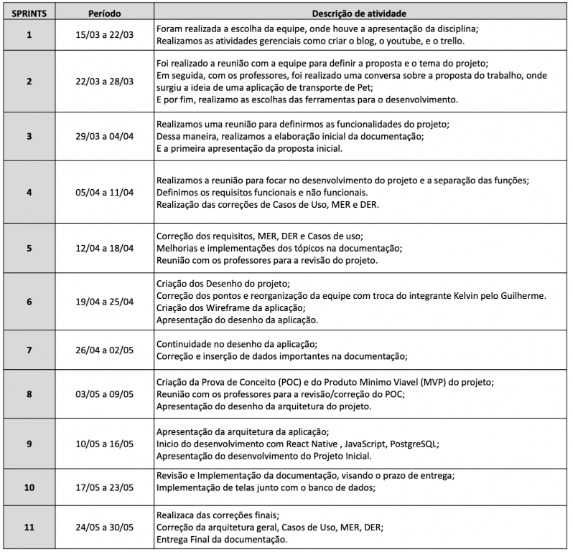
\includegraphics{exemplos/diagramas/Sprints de 11 semanas realizada pela equipe..jpeg}
    \caption{Sprints de 11 semanas realizada pela equipe.}
    \label{fig:Sprints de 11 semanas realizada pela equipe.}
    \fonte {Os Autores}
\end{figure}
% ----------------------------------------------------------
%WIREFRAME
\chapter{Wireframe}
\begin{center}
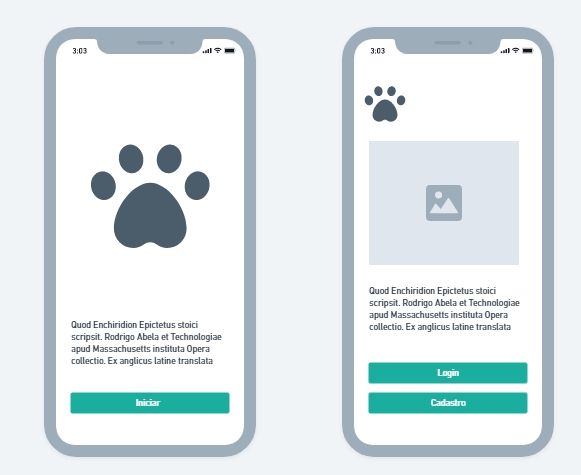
\includegraphics[width=230]{exemplos/Wireframe/Wireframe1.PNG}
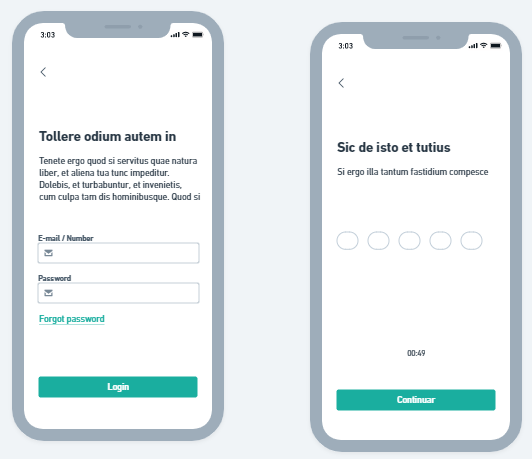
\includegraphics[width=220]{exemplos/Wireframe/Wireframe2.PNG}
\\
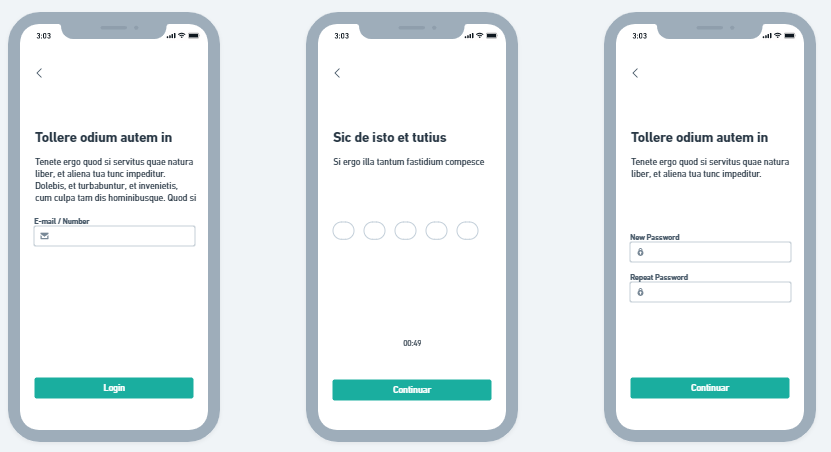
\includegraphics[width=250]{exemplos/Wireframe/Wireframe3.PNG}

\includegraphics[width=100]{exemplos/Wireframe/Wireframe4.PNG}
\\
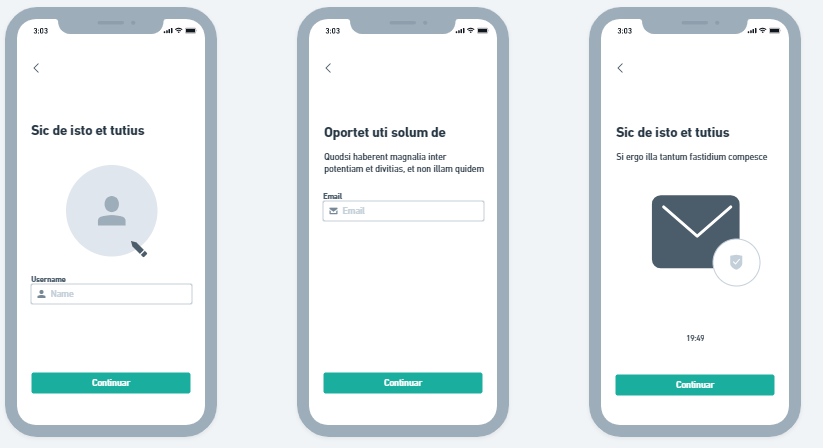
\includegraphics[width=250]{exemplos/Wireframe/Wireframe5.PNG}
\\
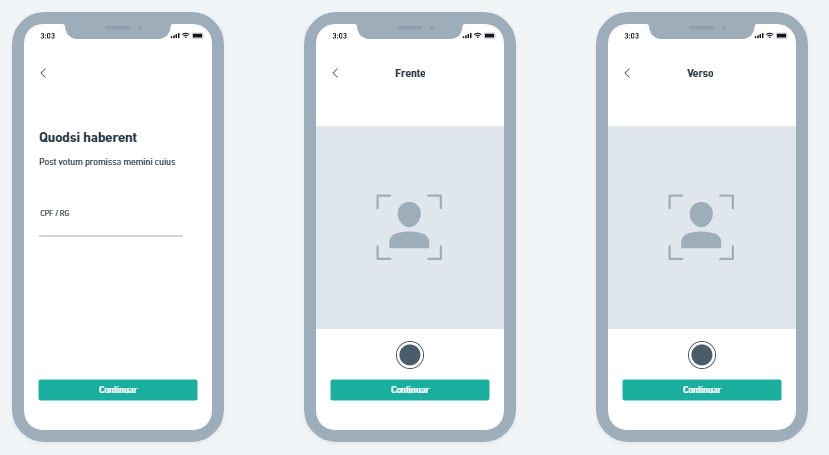
\includegraphics[width=250]{exemplos/Wireframe/Wireframe6.PNG}
\\
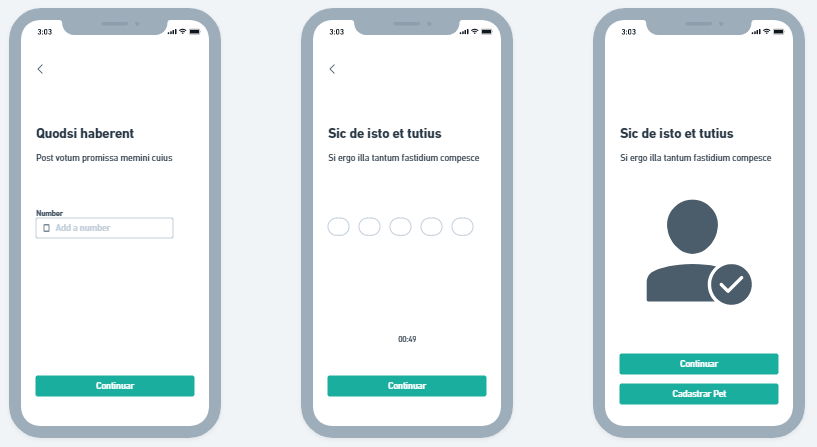
\includegraphics[width=250]{exemplos/Wireframe/Wireframe7.PNG}

\includegraphics[width=100]{exemplos/Wireframe/Wireframe7_1.PNG}
\\
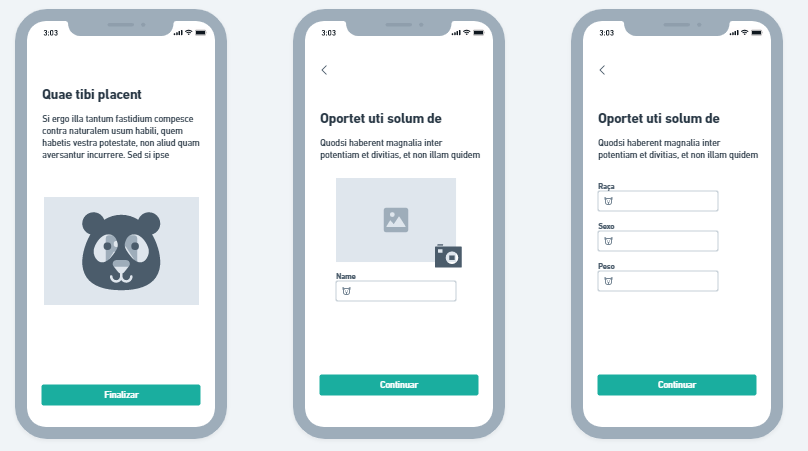
\includegraphics[width=250]{exemplos/Wireframe/Wireframe8.PNG}
\\
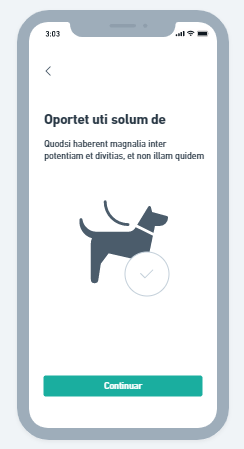
\includegraphics[width=200]{exemplos/Wireframe/Wireframe9.PNG}
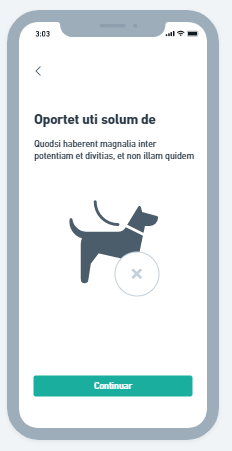
\includegraphics[width=200]{exemplos/Wireframe/Wireframe10.PNG}
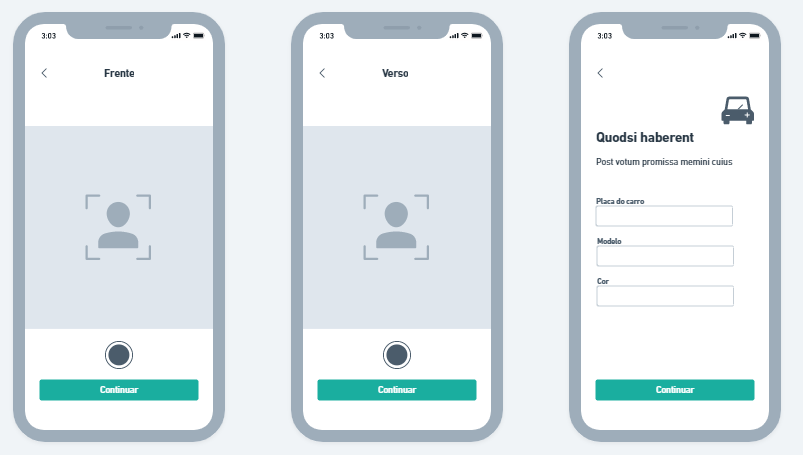
\includegraphics[width=200]{exemplos/Wireframe/Wireframe11.PNG}
\\
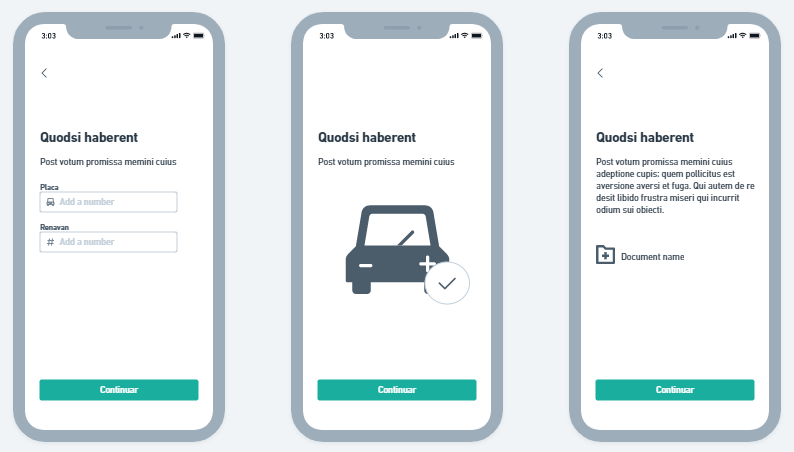
\includegraphics[width=200]{exemplos/Wireframe/Wireframe12.PNG}
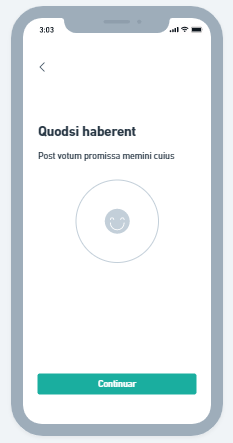
\includegraphics[width=80]{exemplos/Wireframe/Wireframe13.PNG}
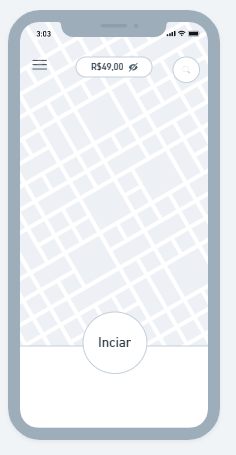
\includegraphics[width=80]{exemplos/Wireframe/Wireframe14.PNG}
\\
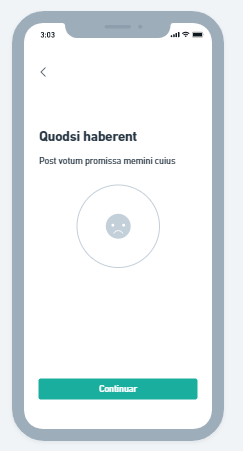
\includegraphics[width=80]{exemplos/Wireframe/Wireframe15.PNG}
\end{center}

% ----------------------------------------------------------
\chapter{HISTÓRIA DE USUÁRIO }
% ----------------------------------------------------------


%REQUISITOS 
\chapter{Requisitos funcionais e não funcionais}

\section{Requisitos funcionais}
\begin{quadro}[thb]
\ABNTEXfontereduzida
\caption{Requisitos Funcionais}
\label{quadro-poluido-limpo-desalinhado}
\begin{tabular}{|l|p{2cm}|l|l|l|p{6cm}|}
\hline
\thead{RF}&\thead{Requisitos\\Funcionais} & \thead{Essencial} & \thead{Importante} & \thead{Desejável} & \thead{Descrição}\\
\hline
RF001&Permitir cadastro de usuários&\circlemark& & & O sistema tem que conceder o cadastro do usuário;\\
\hline
RF002&Permitir cadastro de usuários com conta Google&\circlemark& & & A aplicação deverá permitir que o usuário se cadastre usando a conta Google.\\
\hline
RF003&Permitir cadastro dos Pets&\circlemark& & & O sistema carece que o usuário realize o cadastro do pet (cachorro ou gato).\\
\hline
RF004&Permitir o cadastro do motorista&\circlemark& & & O app deverá aceitar o cadastro do motorista;\\
\hline
RF005&Validar e-mail&\circlemark& & & A aplicação precisa validar se o e-mail informado está correto, enviando um e-mail para o tipo usuário que está solicitando o cadastro. No máximo em 10 segundos.\\
\hline
RF006&Validar celular&\circlemark& & & A aplicação deve enviar um sms validando o número do celular do cliente cadastrado e do motorista no máximo em 10 segundos.\\
\hline
RF007&Realizar o login &\circlemark& & & O sistema deverá permitir o usuário efetuar login;\\
\hline
RF008&Escolher modalidade&\circlemark& & & Quando o cliente acessar o aplicativo o cliente escolher a modalidade comum ou premium, sendo a modalidade comum somente transporte de levar até um local específico e a premium disponibiliza serviços como: transporte e cuidado em parque, acompanhamento no veterinário e etc.\\
\hline
RF009&Quantidade de pets&\circlemark& & & A aplicação deverá solicitar que o cliente informe a quantidade de pets que irá ser transportado;\\
\hline
RF010&Escolher forma de pagamento&\circlemark& & & O cliente define a forma de pagamento como: cartão de crédito com cobrança na hora ou dinheiro depositado previamente na conta.\\
\hline
\end{tabular}
\fonte{Os autores.}
\end{quadro}

\newpage
\begin{quadro}[thb]
\ABNTEXfontereduzida
\begin{tabular}{|l|p{2cm}|l|l|l|p{6cm}|}
\hline
\thead{RF}&\thead{Requisitos\\Funcionais} & \thead{Essencial} & \thead{Importante} & \thead{Desejável} & \thead{Descrição}\\
\hline
RF011&Calcular viagem&\circlemark& & & A aplicação deverá informar ao cliente o valor da viagem antes do mesmo iniciar a viagem, levando em consideração a quantidade de pets, distância e modalidade (serviços da modalidade premium);\\
\hline
RF012&Informar tempo estimado da chegada do veículo&\circlemark& & & Através de um cálculo utilizando distância entre o passageiro e o motorista, o sistema deverá estimar um tempo de chegada. \\
\hline
RF013&Solicitar Transporte &\circlemark& & & O sistema deverá possibilitar a um usuário com perfil passageiro informar um local de origem e destino, para posteriormente fazer uma solicitação de transporte. \\
\hline
RF014&Acompanhar o pet no mapa&\circlemark& & & Tanto os passageiros como motoristas deverão poder acompanhar a posição do usuário que estiverem envolvidos na viagem.\\
\hline
RF015&Conversar com o motorista&\circlemark& & & A aplicação precisa disponibilizar  um chat para a comunicação entre o cliente e o motorista;\\
\hline
RF016&Agendar viagem& &\circlemark& & Descrição: A aplicação deverá disponibilizar a disponibilidade do motorista para o cliente, caso o mesmo deseje agendar uma nova viagem previamente.\\
\hline
RF017&Permitir confirmação da viagem&\circlemark& & & Toda viagem necessita ser confirmada tanto pelos passageiros como motoristas. \\
\hline
RF018&Finalizar viagem&\circlemark& & & A aplicação só liberará a opção de finalizar a viagem ao motorista a 1 metro do final do trajeto;\\
\hline
RF019&Permitir cancelamento da viagem&\circlemark& & & O cancelamento só será permitido caso houver um incidente pelo motorista. O sistema mostrará uma tela informando os possíveis motivos para o cancelamento.\\
\hline
RF20&Realizar avaliação da viagem&\circlemark& & & Ao término de cada viagem o passageiro irá receber uma mensagem no celular para estar avaliando a experiência da viagem e do serviço feito pelo motorista. \\
\hline
\end{tabular}
\fonte{Os autores.}
\end{quadro}
\\

%-----------------------------------------------%
\newpage
\\
\section{Requisitos não funcionais}
\begin{quadro}[thb]
\ABNTEXfontereduzida
\caption{Requisitos não funcionais}
\label{quadro-poluido-limpo-desalinhado}
\begin{tabular}{|l|p{2cm}|l|l|l|p{6cm}|}
\hline
\thead{RNF}&\thead{Requisitos\\Funcionais} & \thead{Essencial} & \thead{Importante} & \thead{Desejável} & \thead{Descrição}\\
\hline
RNF001&Interface com boa usabilidade&\circlemark& & & A aplicação deve ser intuitiva, de modo que possa ser de fácil entendimento  a todas as pessoas que acessarem o aplicativo.\\
\hline
RNF002&Resposta rápida do servidor&\circlemark& & & O software tem que fazer as consultas, histórico de viagens e a autenticação em menos de 1 segundo no lado do servidor.\\
\hline
RNF003&Verificar senha&\circlemark& & & O aplicativo necessita validar se a senha é composta por letras,caracteres especiais e número.\\
\hline
RNF004&Viagem acompanhada com o dono& &\circlemark& & O cliente deve informar via aplicativo para o motorista se irá acompanhar o seu pet. (haverá um botão no app) .\\
\hline
RNF005&Exibir senha& &\circlemark& & O aplicativo deve disponibilizar a opção de visualizar a senha.\\
\hline
RNF006&Disponibilidade do aplicativo&\circlemark& & & A aplicação deve estar disponível 99,99\% do tempo para os usuários, sete dias por semana e 24 horas por dia.\\
\hline
RNF007&Restringir a quantidade de  pets&\circlemark& & & O sistema deve informar a quantidade máxima de pets que o motorista pode transportar, tendo o máximo de 4 pets. \\
\hline
\end{tabular}
\fonte{Os autores.}
\end{quadro}


% ----------------------------------------------------------
\chapter{REGRA DE NEGÓCIOS}
% ----------------------------------------------------------


\end{apendicesenv}
% ---
